\section{稳定性与长期行为}
\label{sec:ctsp-stability}

长时间运行之后会发生什么？这个问题对随机系统有两种不同的问法。第一种沿用第~\ref{chap:ordinary-differential-equations}章的视角：把同一噪声下的两条解放在一起，问初值扰动是否衰减，平衡点是否吸引附近的路径。第二种是第~\ref{chap:discrete-time-stochastic-processes}章的视角：不看单条路径，问状态的分布是否趋于一个不变分布，时间平均是否趋于总体平均。OU过程的路径不收敛到任何点，分布却收敛；乘性噪声的线性方程几乎每条路径都趋于零，二阶矩却可能发散。本节把这些情形分开讨论。

\subsection{随机状态的稳定性}
\label{sec:ctsp-stochastic-stability}

\paragraph{同一噪声下的两条解}
比较初值扰动的影响，最直接的办法是用同一条Brownian路径驱动两个初值。对加性噪声的线性方程$\mathrm dX=-\lambda X\,\mathrm dt+\sigma\,\mathrm dW$，两条解之差满足$\mathrm d(X^x-X^y)=-\lambda(X^x-X^y)\,\mathrm dt$，噪声完全抵消，$X^x_t-X^y_t=e^{-\lambda t}(x-y)$。初值的影响按确定性的速率消失，而每条路径仍在不断波动。

若噪声依赖状态，差也会带上噪声。设$\bm b(\bm0)=\bm0$、$\bm\sigma(\bm0)=\bm0$，于是$\bm0$是一个平衡解：从零出发的路径永远停在零。问题是附近的路径是否被吸引到零。随机情形有几种不等价的稳定要求，需要分别命名。
\begin{itemize}
  \item \term{依概率稳定}（stability in probability）：对任意$\varepsilon,\eta>0$，存在$\delta>0$，使$\|\bm x\|_2<\delta$时$\mathbb P_{\bm x}(\sup_{t\geq0}\|\bm X_t\|_2>\varepsilon)<\eta$。
  \item \term{几乎必然指数稳定}（almost sure exponential stability）：存在$\kappa>0$，使对所有初值，$\limsup_{t\to\infty}t^{-1}\log\|\bm X_t\|_2\leq-\kappa$几乎必然。
  \item $p$阶\term{矩指数稳定}（moment exponential stability），其中$p>0$：存在$C,\kappa>0$，使$\mathbb E_{\bm x}\|\bm X_t\|_2^p\leq C\|\bm x\|_2^pe^{-\kappa t}$；$p=2$时称均方指数稳定。
\end{itemize}

\paragraph{标量乘性噪声}
最简单的例子已经把这几种稳定区分开了。考虑$\mathrm dX=bX\,\mathrm dt+\sigma X\,\mathrm dW$，$X_0=x\neq0$。由第~\ref{sec:ctsp-linear-sde}节的几何Brownian运动公式，$X_t=x\exp\{(b-\sigma^2/2)t+\sigma W_t\}$，于是
\begin{equation}
  \frac1t\log|X_t|=\frac{\log|x|}t+b-\frac{\sigma^2}2+\sigma\frac{W_t}t\longrightarrow b-\frac{\sigma^2}2\quad\text{几乎必然},
  \label{eq:ctsp-lyapunov-exponent}
\end{equation}
\begin{equation}
  \mathbb E|X_t|^p=|x|^p\exp\Bigl\{p\Bigl(b+\frac{(p-1)\sigma^2}2\Bigr)t\Bigr\}.
  \label{eq:ctsp-pth-moment}
\end{equation}
第二式由$\mathbb Ee^{p\sigma W_t}=e^{p^2\sigma^2t/2}$得到。几乎必然指数稳定当且仅当$b<\sigma^2/2$，均方指数稳定当且仅当$2b+\sigma^2<0$。

取$b=-1$、$\sigma^2=3$。无噪声时$\dot x=-x$稳定；加噪声后，几乎必然指数为$-2.5$，路径比无噪声时衰减得更快，但二阶矩指数为$2b+\sigma^2=1>0$，$\mathbb EX_t^2$指数增长。图~\ref{fig:ctsp-multiplicative-stability}画出了这一对照：每条路径的$\log|X_t|$都沿斜率$-2.5$下降，均方却在上升。原因是$\log X_t$服从正态分布，$X_t^2$是对数正态的，它的期望由极少数极大值支配；这些路径出现的概率随时间迅速变小，但它们对二阶矩的贡献增长得更快。反过来，$b=0.5$、$\sigma=1.5$时，确定性部分不稳定，几乎必然指数却是$0.5-1.125<0$：噪声使路径几乎必然衰减。所以“确定性部分稳定”既不是随机稳定的充分条件，也不是必要条件，而且不同稳定概念需要分别检查。

\begin{figure}[htbp]
  \centering
  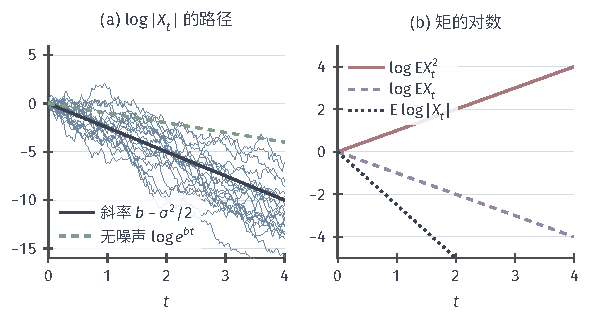
\includegraphics[width=100mm]{figures/03-optimization-evolution-and-signals/02-processes-and-trajectory-evolution/tikz/ctsp-multiplicative-stability/figure.pdf}
  \caption{乘性噪声下几乎必然稳定与均方不稳定并存。模型$\mathrm dX=bX\,\mathrm dt+\sigma X\,\mathrm dW$，$b=-1$，$\sigma^2=3$，$X_0=1$。(a)$20$条路径的$\log|X_t|$（由显式解在网格上生成，固定随机种子），黑线为斜率$b-\sigma^2/2=-2.5$，绿虚线为无噪声解；(b)解析的矩指数：$\log\mathbb EX_t^2=(2b+\sigma^2)t$上升，$\log\mathbb EX_t=bt$与$\mathbb E\log|X_t|=(b-\sigma^2/2)t$下降。}
  \label{fig:ctsp-multiplicative-stability}
\end{figure}

式~\eqref{eq:ctsp-pth-moment}还揭示了两类稳定之间的联系。矩指数$p(b+(p-1)\sigma^2/2)$在$p=0$处为零，对$p$的导数为$b-\sigma^2/2$，恰为几乎必然指数。所以几乎必然指数稳定当且仅当对充分小的$p>0$有$p$阶矩指数稳定；阶数越高，越容易被罕见的大值破坏。

\paragraph{随机Lyapunov函数}
没有显式解时，第~\ref{chap:ordinary-differential-equations}章的Lyapunov方法仍然可用，只是沿路径的导数要换成Itô公式的漂移，即生成元$\mathcal LV$。

\begin{theorem}[矩稳定的Lyapunov判据]
  \label{thm:ctsp-lyapunov-moment}
  设系数局部Lipschitz，$\bm b(\bm0)=\bm0$，$\bm\sigma(\bm0)=\bm0$。若存在$V\in C^2(\mathbb R^d)$与常数$c_1,c_2,c_3>0$、$p>0$，使
  \[
    c_1\|\bm x\|_2^p\leq V(\bm x)\leq c_2\|\bm x\|_2^p,\qquad\mathcal LV(\bm x)\leq-c_3V(\bm x)
  \]
  对所有$\bm x$成立，则解不爆炸，并且$\mathbb E_{\bm x}\|\bm X_t\|_2^p\leq(c_2/c_1)\|\bm x\|_2^pe^{-c_3t}$，即零解$p$阶矩指数稳定。
\end{theorem}

\begin{proof}
不爆炸由定理~\ref{thm:ctsp-nonexplosion}（取常数$c=0$）得到。对$U(t,\bm x)=e^{c_3t}V(\bm x)$使用含时间的Itô公式，漂移为$e^{c_3t}(c_3V+\mathcal LV)\leq0$。在$\tau_R\wedge t$停止，随机积分期望为零，$\mathbb E[e^{c_3(\tau_R\wedge t)}V(\bm X_{\tau_R\wedge t})]\leq V(\bm x)$；令$R\to\infty$，Fatou引理给出$\mathbb E[e^{c_3t}V(\bm X_t)]\leq V(\bm x)$，再代入$V$的上下界。
\end{proof}

以标量乘性模型核对：$V(x)=x^2$时$\mathcal LV=(2b+\sigma^2)x^2$，判据给出均方稳定当且仅当$2b+\sigma^2<0$，与显式计算一致。判据的证明串起了本章前面的几步：局部Lipschitz给出到爆炸为止的解，Lyapunov函数排除爆炸，含时间的Itô公式与停止保证期望可以取，Fatou引理去掉截断。几乎必然稳定可以用同样的思路处理$\log V$，但所需条件不同，须另行检查；不同的结论对应不同的函数控制与噪声条件，不能笼统地称为“稳定”。

\subsection{不变分布与分布趋稳}
\label{sec:ctsp-invariant}

\paragraph{半群的不动点}
离散章区分了三件事：不变分布存在，不变分布唯一，从给定初值出发的分布收敛到它。连续时间的不变性写成对所有时长同时成立的不动点条件：若
\[
  \mu P_t=\mu\qquad\text{对所有 }t\geq0 ,
\]
就称$\mu$为\term{不变分布}（invariant distribution）。以$\mu$为初始分布的过程在每个时刻都有同样的边缘分布，并且由时间齐次性，整个过程关于时间平移的联合规律不变。

验证不变性时，通常不直接计算$\mu P_t$，而检查生成元。由弱形式~\eqref{eq:ctsp-weak-evolution}，若$\mu$不变，则$\int\mathcal Lf\,\mathrm d\mu=0$对所有$f\in C^2_c$成立；有密度时等价于Fokker--Planck方程的稳态$\mathcal L^*p=0$。反方向需要更多条件：$\int\mathcal Lf\,\mathrm d\mu=0$只是候选，要推出$\mu P_t=\mu$，还需鞅问题适定，或$C^2_c$在生成元定义域中足够丰富。连续时间Markov链中这一检验就是$\bm\pi\bm Q=\bm0$；可数状态时还要求链不爆炸。

\paragraph{OU过程的稳态}
OU过程可以把候选验证与实际收敛都算出来。第~\ref{sec:ctsp-backward-forward}节由稳态Fokker--Planck方程得到候选$\pi=\mathcal N(0,\sigma^2/(2\lambda))$。实际收敛由显式解给出：$X_t=e^{-\lambda t}X_0+Z_t$，其中$Z_t=\sigma\int_0^te^{-\lambda(t-s)}\,\mathrm dW_s\sim\mathcal N(0,\sigma^2(1-e^{-2\lambda t})/(2\lambda))$与$X_0$独立。第一项几乎必然趋于零，第二项的分布趋于$\pi$，所以对任何初值分布，$X_t$的分布都收敛到$\pi$，$\pi$也因此是唯一的不变分布。

收敛速度可以用同一噪声的耦合读出。两个从不同初值出发、由同一$W$驱动的解满足$|X^x_t-X^y_t|=e^{-\lambda t}|x-y|$。若让$X^y_0$服从$\pi$，它在所有时刻都服从$\pi$，于是$X^x_t$与一个服从$\pi$的变量之间的均方距离不超过$e^{-\lambda t}(\mathbb E|x-X^y_0|^2)^{1/2}$。这个耦合给出分布之间按速率$\lambda$的指数收敛：二阶Wasserstein距离定义为两个分布的所有耦合下均方根距离的下确界，所以它不超过上面这个特定耦合给出的$e^{-\lambda t}(\mathbb E|x-X^y_0|^2)^{1/2}$。这一距离及其性质可参考\BookChapterRef{chap:information-theory-and-statistical-geometry}{卷四“信息论与统计几何”章}。

\paragraph{一般扩散还需检查什么}
形式上解出稳态方程$\mathcal L^*p=0$，离得到“过程收敛到$p$”还有好几步，每一步都可能失败。
\begin{itemize}
  \item 解可能不可归一化。Brownian运动的生成元$\frac12\partial_{xx}$满足$\int\mathcal Lf\,\mathrm dx=0$，Lebesgue测度是不变测度，但它不是概率分布；Brownian运动没有不变分布，$W_t$的分布不断摊开。
  \item 不变分布可能不唯一。设$\mathrm dX=X(1-X)\,\mathrm dW$，$X_0\in[0,1]$：噪声在$0$与$1$处消失，$\delta_0$与$\delta_1$都是不变分布，路径最终被吸收到其中一个端点，吸收到哪一个取决于初值。扩散退化使过程不可约性失败。
  \item 过程本身可能不良定，例如在有限时间爆炸，或在有界区域上缺少与模型一致的边界条件。
\end{itemize}
一组常用的充分条件是：系数光滑，扩散一致椭圆，并且存在随状态增长而趋于无穷的Lyapunov函数$V$，使$\mathcal LV\leq-cV+d$（$c>0$）。前者保证过程能以正概率到达各处，因而至多一个不变分布；后者把过程拉回有界区域，保证不变分布存在并且从任何初值出发的分布收敛到它\scite{math-meyn2009markov}。存在、唯一与收敛应分别论证，不能由形式稳态密度直接推出。

\subsection{连续时间平均与波动}
\label{sec:ctsp-time-average}

\paragraph{时间平均的遍历定理}
离散章的遍历定理说，平稳遍历时$n^{-1}\sum_{k<n}f(X_k)$几乎必然趋于$\int f\,\mathrm d\pi$。连续时间把样本平均换成单位时间的累计
\begin{equation}
  \bar f_T=\frac1T\int_0^Tf(X_t)\,\mathrm dt .
  \label{eq:ctsp-time-average}
\end{equation}
渐进可测性保证积分是随机变量。若$X$以不变分布$\pi$启动且平稳过程是遍历的，对$\pi$可积的$f$有$\bar f_T\to\int f\,\mathrm d\pi$几乎必然；对满足适当回返条件（例如正Harris常返）的Markov过程，结论对任意初值成立\scite{math-meyn2009markov}。OU过程中，$\bar X_T\to0$，$\overline{X^2}_T\to\sigma^2/(2\lambda)$。

一个自然的捷径是只在等间隔时刻$kh$观察，把连续时间问题化为离散链$(X_{kh})_k$，称为\term{骨架链}（skeleton chain）。骨架链的不变分布包含连续过程的不变分布，但遍历性不一定传递。确定性的例子最清楚：单位圆上的匀速旋转$X_t=(\cos t,\sin t)$，均匀分布不变，连续时间平均对任何连续函数都收敛到均匀分布下的平均；取$h=2\pi$，骨架链却停在原地，样本平均只是初值处的函数值。随机过程中扩散非退化通常能排除这种共振，但需要检查，而不是默认骨架链与连续过程等价。

\paragraph{长期方差与Poisson方程}
遍历定理只说平均会收敛，不说误差有多大。设$X$平稳，$f$平方可积，记$C(s)=\operatorname{Cov}_\pi(f(X_0),f(X_s))$。由平稳性与Fubini定理，
\[
  \operatorname{Var}\Bigl(\int_0^Tf(X_t)\,\mathrm dt\Bigr)=\int_0^T\!\!\int_0^TC(|t-s|)\,\mathrm ds\,\mathrm dt=2\int_0^T(T-s)C(s)\,\mathrm ds .
\]
若$\int_0^\infty|C(s)|\,\mathrm ds<\infty$，则$T\operatorname{Var}(\bar f_T)\to\sigma_f^2=2\int_0^\infty C(s)\,\mathrm ds$，极限$\sigma_f^2$称为\term{长期方差}（asymptotic variance）。这与离散章的协方差和相对应：相关越持久，有效的独立观测越少。OU过程取$f(x)=x$，$C(s)=\frac{\sigma^2}{2\lambda}e^{-\lambda s}$，于是$\sigma_f^2=\sigma^2/\lambda^2$。

中心极限定理需要比方差公式更多的结构。一条有用的路线是解Poisson方程：找$g$使
\begin{equation}
  -\mathcal Lg=f-\int f\,\mathrm d\pi .
  \label{eq:ctsp-poisson-equation}
\end{equation}
对$g(X_t)$使用Itô公式，$g(X_T)-g(X_0)=\int_0^T\mathcal Lg(X_t)\,\mathrm dt+M_T$，其中$M_T=\int_0^T\nabla g^\top\bm\sigma\,\mathrm d\bm W$。整理得
\[
  \int_0^T\Bigl(f(X_t)-\int f\,\mathrm d\pi\Bigr)\mathrm dt=g(X_0)-g(X_T)+M_T .
\]
时间平均的误差被拆成有界的边界项与一个鞅。若$g$满足适当的矩条件，边界项除以$\sqrt T$后趋零，鞅的中心极限定理给出$\sqrt T(\bar f_T-\int f\,\mathrm d\pi)\Rightarrow\mathcal N(0,\sigma_f^2)$，其中$\sigma_f^2=\int\|\bm\sigma^\top\nabla g\|_2^2\,\mathrm d\pi$，即鞅的平均二次变差速率。仍以OU过程、$f(x)=x$核对：$g(x)=x/\lambda$满足$-\mathcal Lg=-(-\lambda x)/\lambda=x$，$\sigma_f^2=\sigma^2/\lambda^2$，与协方差积分的结果一致。

这条路线的每一步都依赖条件：Poisson方程可解，解有足够的矩，鞅中心极限定理的条件成立。遍历性本身不保证这些，连续时间的遍历过程也可以没有中心极限定理。第~\ref{sec:ctsp-sampling}节用这里的长期方差为时间平均估计标准误；协方差函数的频谱表示与估计留给第~\ref{chap:signal-analysis}章。
